% !TEX program = xelatex
% ============================================================================
%  暨南大学经济学院  Beamer 模板
%  ---------------------------------------------------------------------------
%  主题   : CambridgeUS（beamer 中 Cambridge 主题的正式名称）
%  配色   : beaver 色，即 #8C0000
%  字体   : Utopia（fourier 宏包）
%  首页   : 顶部栏 + 圆角标题框（beaver 底 + 白色文字）+ 作者/机构/日期
%           + TikZ 绘制的 #8C0000 矩形承载院徽 + 底部三段式信息表
%  编译   : xelatex（中文需要 ctex，请用 XeLaTeX 编译两次以生成页码/书签）
% ============================================================================
\documentclass[aspectratio=169, 11pt]{ctexbeamer}
%  需要 4:3 时把上面换成：
%  \documentclass[11pt]{ctexbeamer}
%  在 macOS / Linux 上编译时，可在导言区加 \ctexset{fontset=fandol}

\usetheme{CambridgeUS}      % Cambridge 主题（含 rounded 内部主题 + infolines 外部主题）
\usecolortheme{beaver}      % CambridgeUS 的默认配色主题

\usepackage{amsmath}
\usepackage{booktabs}        % 三线表的 \toprule / \midrule / \bottomrule
\usepackage{tikz}

% 图片统一放在仓库根目录的 image/ 里（本 .tex 位于
% “暨南大学经济学院Beamer模板/”子目录内，所以图片在 ../image/）。
% 两个路径都写上，这样在本目录里编译、或在仓库根目录里编译都能找到图片。
\graphicspath{{../image/}{image/}}

% 编译：请先 cd 进本目录（图片与 .bib 都按相对路径查找），然后
%   xelatex jnu_beamer_template.tex   →   bibtex jnu_beamer_template
%     →   xelatex jnu_beamer_template.tex   ×2

% ---------------------------------------------------------------------------
% 1. 字体：Utopia
%    fourier 宏包提供 Utopia 文本字体和配套的 Fourier 数学字体。
%    beamer 默认用无衬线字体，\usefonttheme{serif} 把正文切到衬线族，
%    正文与标题即为 Utopia；professionalfonts 让 beamer 不要替换数学字体。
%    注意：切换衬线族后，中文会跟着走 \rmfamily，即 ctex 的 CJK 主字体（宋体）。
%    若希望中文仍用黑体，取消下一行注释即可。
% ---------------------------------------------------------------------------
\usepackage{fourier}
\usefonttheme{serif}
\usefonttheme{professionalfonts}
% \setCJKmainfont{SimHei}

% ---------------------------------------------------------------------------
% 2. 颜色：定义主题色 beaver = #8C0000
%    beamer 只提供 beaver 配色主题，并未定义同名的 beaver 颜色，故在此定义。
%    作者、机构、日期一律沿用主题默认颜色，这里不做改动。
%    （beamer 默认配色并未给 author / institute / date 设色，所以它们取正文
%      颜色，即黑色；beaver 配色主题只设了 titlelike / title，不含这三个。）
% ---------------------------------------------------------------------------
\definecolor{beaver}{RGB}{140,0,0}          % #8C0000

% 标题框用 beaver 底 + 白色文字；副标题与标题同框，故一并设为白色
\setbeamercolor{title}     {fg=white, bg=beaver}
\setbeamercolor{subtitle}  {fg=white, bg=beaver}

% itemize 项目符号的前景色用 beaver
\setbeamercolor{item}{fg=beaver}
% 需要二、三级符号也同样处理时，取消下面两行注释
% \setbeamercolor{subitem}{fg=beaver}
% \setbeamercolor{subsubitem}{fg=beaver}

% 去掉每页右下角默认的导航图标，页脚只保留 infolines 的三段式信息表
\setbeamertemplate{navigation symbols}{}

% ---------------------------------------------------------------------------
% 3. 标题 / 副标题 / 作者：均不加粗
%    标题、副标题字号比 beamer 默认小一档；作者只保留 \large 字号。
%    作者 / 机构 / 日期不设 fg，颜色即主题默认（黑色）。
% ---------------------------------------------------------------------------
\setbeamerfont{title}     {size=\Large, series=\mdseries}
\setbeamerfont{subtitle}  {size=\normalsize, series=\mdseries}
\setbeamerfont{author}    {size=\large, series=\mdseries}
\setbeamerfont{institute} {size=\normalsize}
\setbeamerfont{date}      {size=\small}

% ---------------------------------------------------------------------------
% 4. 院徽矩形：尺寸与内边距
%    院徽原图（jnu_econ_logo_white.png）宽高比为 4045 : 721，尺寸按此比例推算
% ---------------------------------------------------------------------------
\newcommand{\jnulogofile}{jnu_econ_logo_white.png}
\newlength{\jnulogowidth}
\newlength{\jnulogoheight}
\newlength{\jnulogopad}
\setlength{\jnulogowidth}{6cm}       % 矩形内院徽的宽度
\setlength{\jnulogopad}{5pt}         % 院徽四周留出的红色边距
% 先除以再乘以宽高比，避免 \dimexpr 中间结果超出 TeX 的尺寸上限
\setlength{\jnulogoheight}{\dimexpr\jnulogowidth/4045*721\relax}

% ---------------------------------------------------------------------------
% 5. 自定义首页（title page）模板
%    两处 \vspace{8mm} 是标题框与作者块、作者块与院徽之间的纵向间距，
%    当前取值按“标题单行”调平（三段间距约 9.9 / 8.5 / 7.8 mm）；
%    若标题换成多行，可据此调小这两个 8mm。
% ---------------------------------------------------------------------------
\makeatletter
\defbeamertemplate*{title page}{jnu}[1][]{%
  \centering
  \vspace*{0.5em}
  % ---- 圆角标题框：主标题 + 子标题 ----
  \begin{beamercolorbox}[sep=12pt, center, rounded=true, shadow=false, wd=\textwidth]{title}
    {\usebeamerfont{title}\inserttitle\par}
    \ifx\insertsubtitle\@empty\else
      \vspace{0.4em}
      {\usebeamerfont{subtitle}\usebeamercolor[fg]{subtitle}\insertsubtitle\par}
    \fi
  \end{beamercolorbox}
  \vspace{8mm}
  % ---- 标题框之下：作者 -> 机构 -> 日期（颜色沿用主题默认） ----
  {\usebeamerfont{author}\usebeamercolor[fg]{author}\insertauthor\par}
  \vspace{0.75em}
  {\usebeamerfont{institute}\usebeamercolor[fg]{institute}\insertinstitute\par}
  \vspace{0.5em}
  {\usebeamerfont{date}\usebeamercolor[fg]{date}\insertdate\par}
  \vspace{8mm}
  % ---- 底部：TikZ 绘制的 beaver 色矩形，用于放置院徽 ----
  % \centerline 使这段（垂直模式下的）内容水平居中
  \centerline{%
    \begin{tikzpicture}
      \fill[beaver]
        (0,0) rectangle
        (\dimexpr\jnulogowidth+2\jnulogopad\relax,
         \dimexpr\jnulogoheight+2\jnulogopad\relax);
      \node at (\dimexpr\jnulogowidth/2+\jnulogopad\relax,
                \dimexpr\jnulogoheight/2+\jnulogopad\relax)
        {\includegraphics[width=\jnulogowidth]{\jnulogofile}};
    \end{tikzpicture}%
  }
  \vspace*{0.5em}
}
\makeatother

% ---------------------------------------------------------------------------
% 6. 首页信息
%    方括号内为“短信息”，供页脚（infolines 外部主题）的三段式信息表使用
% ---------------------------------------------------------------------------
\title[The Elements Of Statistical Learning]{The Elements Of Statistical Learning}
\subtitle{The First Lesson}
\author[FU]{FU}
\institute[暨南大学经济学院]{暨南大学经济学院}
\date{2026年9月1日}

% ---------------------------------------------------------------------------
% 7. 图注与编号
%    beamer 默认的 caption 模板只印“图”不印编号，这里换成 numbered 版本；
%    标签分隔符改为全角冒号，中文排版更规范（“图 1：…”）。
%    默认模板里的对齐是 \raggedright（左对齐）；需要居中时，在 frame 内直接
%    \setbeamertemplate{caption}[centered]，表格结束后再改回 [numbered]。
%    不要用 { } 把这组设置包起来做作用域：实测在额外一层组里，表题的颜色会
%    渗进紧跟其后的 tabular，把表格文字染成 #CC0000。
% ---------------------------------------------------------------------------
\setbeamertemplate{caption}[numbered]
\defbeamertemplate{caption label separator}{jnu}{：\hspace{0.15em}}
\setbeamertemplate{caption label separator}[jnu]
% 居中版 caption 模板：与 numbered 版完全相同，只把 \raggedright 换成 \centering
\defbeamertemplate{caption}{centered}{%
  \centering
  {\usebeamercolor[fg]{caption name}\usebeamerfont*{caption name}%
   \insertcaptionname~\insertcaptionnumber
   \usebeamertemplate{caption label separator}}%
  \insertcaption\par
}

% ---------------------------------------------------------------------------
% 8. 参考文献：GB/T 7714-2015 顺序编码制（gbt7714 + BibTeX）
%    条目写在 references.bib 里。gbt7714 内部已经 \RequirePackage{natbib}，
%    所以不需要再单独 \usepackage{natbib}；bibliographystyle 选 -numerical
%    即“顺序编码制”，正文 \cite 输出 [1]、列表自动编号 [1]、[2]、…
%    注意：gbt7714 的 numbers / super / authoryear 选项已废弃，直接用
%    下面的 bibliographystyle 指定即可（实测正文输出就是 [1]，非上标）。
%    \bibliography 默认只列被 \cite 过的条目，参考文献页用 \nocite{*}
%    把 .bib 里的条目全部列出。
%    beamer 默认的 bibliography item 模板什么都不印，这里补上 \insertbiblabel
%    才能把 [1] 显示出来。
%    首次编译（或改动过 .bib 之后）需要跑一遍 bibtex：
%        xelatex 主文件  →  bibtex 主文件  →  xelatex 主文件 ×2
% ---------------------------------------------------------------------------
\usepackage{gbt7714}
\bibliographystyle{gbt7714-numerical}
\setbeamertemplate{bibliography item}{\insertbiblabel}

\begin{document}

% 首页不加 [plain]，顶部栏与底部三段式信息表才会出现
\begin{frame}
  \titlepage
\end{frame}

% ---------------------------------------------------------------------------
% 目录页：\tableofcontents 显示全文的 \section{} / \subsection{}，
% 章节写在它后面也能被收进来；新增或改动章节后要编译两遍才会更新。
% ---------------------------------------------------------------------------
\begin{frame}{目录}
  \tableofcontents
\end{frame}

% ===========================================================================
%  以下为示例页面，用于预览模板效果，可按需删除
% ===========================================================================
\section{示例}

\begin{frame}{示例页面}
  \begin{itemize}
    \item 正文使用 CambridgeUS 主题默认样式，强调色为主题色 beaver。
    \item 关键结论可以用 \alert{主题色高亮} 标出。
    \item 中文由 ctex 提供支持，请使用 XeLaTeX 编译。
  \end{itemize}
  \vspace{0.6em}
  \begin{block}{圆角区块}
    区块样式来自 CambridgeUS 主题内置的 rounded 内部主题。
  \end{block}
\end{frame}

% ---------------------------------------------------------------------------
% 数学公式页：上方配图 + 自动编号图注（图高 3.4cm），下方只放一个优化目标公式。
% 图注编号来自导言区第 7 节的 \setbeamertemplate{caption}[numbered]。
% 配图为 LR.png 去掉白边后的 LR_trim.png。
% ---------------------------------------------------------------------------
\section{数学公式}

\begin{frame}{数学公式}
  \begin{figure}
    \centering
    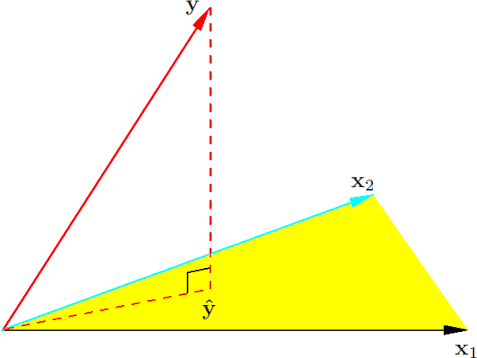
\includegraphics[height=3.4cm]{LR_trim.png}
    \caption{线性回归的几何视角}
  \end{figure}
  \[
    \min_{\boldsymbol{\beta}}\|\boldsymbol{y}-X\boldsymbol{\beta}\|_2^2
    =
    \min_{\boldsymbol{\beta}}\sum_{i=1}^{n}(y_i-\hat{y}_i)^2
  \]
\end{frame}

% ---------------------------------------------------------------------------
% 三线表页：booktabs 三线表（只留顶线 / 中线 / 底线，无竖线），表格居中，
% 三列全部水平居中（tabular 的 ccc）。表题写在表格上方（中文排版惯例），
% 表号自动编号，显示为“表 1：…”；表题居中用上面的 centered caption 变体。
% 注意：不要用 { } 把 table 包起来做作用域。实测在额外一层组里，表题的颜色
% 会渗进紧跟其后的 tabular，把表格文字染成 #CC0000；所以这里直接在本 frame
% 内选用模板，并在表格结束后改回 numbered（模板设置会延续到后面的 frame）。
% 本 frame 不另起 \section，仍属于「数学公式」这一节。
% ---------------------------------------------------------------------------
\begin{frame}{三线表}
  \setbeamertemplate{caption}[centered]%
  \begin{table}
    \centering
    \caption{这是一个三线表}
    \begin{tabular}{ccc}
      \toprule
      姓名  & 性别 & 学号 \\
      \midrule
      David & M    & 123  \\
      Alice & F    & 456  \\
      \bottomrule
    \end{tabular}
  \end{table}
  \setbeamertemplate{caption}[numbered]%
\end{frame}

% ---------------------------------------------------------------------------
% 参考文献页：条目由 BibTeX 从 references.bib 生成，GB/T 7714-2015 顺序编码制。
% \nocite{*} 让 .bib 里的条目全部列出（否则 \bibliography 只列被 \cite 过的）。
% \section*{参考文献}：把本页从「数学公式」这一节的逻辑范围里分出来，
% 同时因为带星号，不会写进 .toc，目录里不会多出“参考文献”一条。
% \begin{frame}[t]：t 让正文从页面顶部开始排，且左对齐（不整体垂直居中）。
% 标题仍走本模板的 frametitle（保持样式一致），只是把 default 模板的
% 对齐参数从默认的 left 换成 center，使标题在顶部水平居中。
% 模板设置会延续到后面的 frame，所以 frame 结束后改回 [default]。
% ---------------------------------------------------------------------------
\section*{参考文献}

\setbeamertemplate{frametitle}[default][center]%
\begin{frame}[t]{参考文献}
  \nocite{*}
  \bibliography{references}
\end{frame}
\setbeamertemplate{frametitle}[default]%

\begin{frame}[plain]
  \centering
  \vfill
  % 注意：这里不能用 \usebeamercolor[fg]{title}，因为 title 的前景色是白色
  % （为首页红色标题框而设），在白底上会看不见。
  {\usebeamerfont{title}\Huge\textcolor{beaver}{谢谢！}\par}
  \vfill
\end{frame}

\end{document}
